% !TEX TS-program = pdflatex
% !TEX encoding = UTF-8 Unicode

% This is a simple template for a LaTeX document using the "article" class.
% See "book", "report", "letter" for other types of document.

\documentclass[12pt,a4paper,titlepage]{scrartcl} % use larger type; default would be 10pt

\usepackage[utf8x]{inputenc} % set input encoding (not needed with XeLaTeX)

%%% Examples of Article customizations
% These packages are optional, depending whether you want the features they provide.
% See the LaTeX Companion or other references for full information.

%%% PAGE DIMENSIONS
\usepackage[a4paper]{geometry} % to change the page dimensions
%\geometry{a4paper} % or letterpaper (US) or a5paper or....
\geometry{bottom=3.5cm} % for example, change the margins to 2 inches all round
% \geometry{landscape} % set up the page for landscape
%   read geometry.pdf for detailed page layout information

\usepackage{graphicx} % support the \begin{center}\includegraphics command and options
\usepackage{wrapfig}

% \usepackage[parfill]{parskip} % Activate to begin paragraphs with an empty line rather than an indent

%%% PACKAGES
\usepackage{booktabs} % for much better looking tables
\usepackage{array} % for better arrays (eg matrices) in maths
\usepackage{paralist} % very flexible & customisable lists (eg. enumerate/itemize, etc.)
\usepackage{verbatim} % adds environment for commenting out blocks of text & for better verbatim
\usepackage{subfig} % make it possible to include more than one captioned figure/table in a single float
% These packages are all incorporated in the memoir class to one degree or another...
\usepackage[ngerman]{babel}
\usepackage{pifont} %for symbols (i.e. arrows)
\usepackage{fancyhdr}
%\usepackage{showframe}

%%redifine of emph, see http://tex.stackexchange.com/questions/6754/what-is-the-canonical-way-to-redefine-the-emph-command
\makeatletter
\DeclareRobustCommand{\em}{%
  \@nomath\em \if b\expandafter\@car\f@series\@nil
  \normalfont \else \bfseries \fi}
\makeatother

%%% HEADERS & FOOTERS
%set with fancy layout package
\usepackage{fancyhdr} % This should be set AFTER setting up the page geometry
\pagestyle{fancy} % options: empty , plain , fancy
\renewcommand{\headrulewidth}{0pt} % customise the layout...
\lhead{}\chead{}\rhead{}
\lfoot{}\cfoot{\thepage}\rfoot{}

\setlength{\parindent}{0mm} %set paragraph begin indentation to 0

%%% SECTION TITLE APPEARANCE
\usepackage{sectsty}
\allsectionsfont{\sffamily\mdseries\upshape} % (See the fntguide.pdf for font help)
% (This matches ConTeXt defaults)

%%% ToC (table of contents) APPEARANCE
%\usepackage[nottoc,notlof,notlot]{tocbibind} % Put the bibliography in the ToC
%\usepackage[titles,subfigure]{tocloft} % Alter the style of the Table of Contents
%\renewcommand{\cftsecfont}{\rmfamily\mdseries\upshape}
%\renewcommand{\cftsecpagefont}{\rmfamily\mdseries\upshape} % No bold!

%%% END Article customizations

%%% The "real" document content comes below...

\title{Installation und Einrichtung von Microsoft Windows Server 2008 R2 zu einem Domain Controller}
\author{Sebastian Deußer}
\date{1. April 2014} % Activate to display a given date or no date (if empty),
         % otherwise the current date is printed 
\setcounter{section}{-1}

\begin{document}
\maketitle %title (page)

%header and footer definitions for fancyhdr
\pagestyle{fancy}
\lhead{}
\chead{\leftmark}
\rhead{}
\lfoot{Sebastian Deußer}
\cfoot{}
\rfoot{Seite \thepage}

\noindent

\thispagestyle{fancy}
\tableofcontents

\newpage
\section{Installation von Windows Server 2008 R2}
Vor der Installation von Windows Server 2008 R2 sollten wir erst einmal sicherstellen das man genug freien Platz auf der Festplatte hat, und diese wenn möglich schon einmal vorpartitionieren. Um noch etwas Luft zum arbeiten zu haben reservieren wir mindestens 30 GB.\\
Um die Installation nun zu starten legen wir die Installations-DVD ins Laufwerk ein und bootet von dieser. Das Installationsprogramm ist selbsterklärend, es sollte aber darauf geachten werden die richtige Partition als Installationsziel auszuwählen.\\
Wenn ein anderer Bootloader als der von Windows verwendet wird (wie z.B. grub von Linux) muss dieser nach der Installation wieder hergestellt werden und ggf. einen Booteintrag für Windows Server 2008 R2 hinzugefügt werden.\\
Nun lassen wir Windows noch seine zahlreichen Updates installieren und dann können wir mit den Vorarbeiten beginnen.

\newpage
\section{Vorarbeiten}
Zunächst einmal sollten wir dem Rechner der Domaincontroller werden soll einen Namen zuweisen. Dazu klicken wir mit der rechten Maustaste auf \emph{Computer} und wählen \emph{Eigenschaften}. Hier wird der Computername angezeigt. Um ihn zu ändern klicken wir die Schaltfläche \emph{Einstellungen ändern} (roter Kasten) an.

	\begin{center}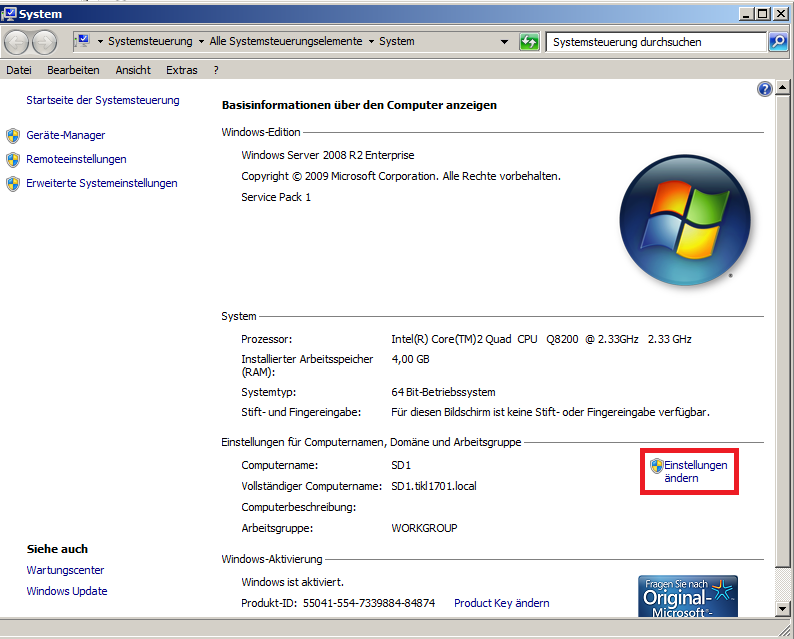
\includegraphics[width=14cm]{Bilder/001(Kasten)}\\ \end{center}

%\newpage
Daraufhin erscheint folgender Dialog:\\

	\begin{center}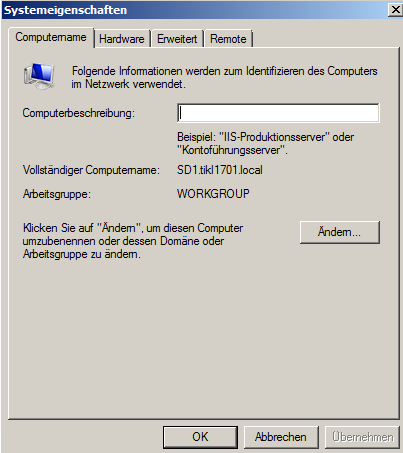
\includegraphics[height=7cm]{Bilder/002}\\ \end{center}
		
Hier können wir mit der Schaltfläche \emph{ändern} einen anderen Computernamen angeben.\\

	\begin{center}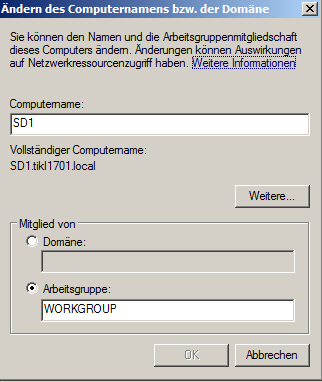
\includegraphics[height=7cm]{Bilder/003}\\ \end{center}
		
Die Arbeitsgruppe kann auf dem Standard belassen werden da dies später bei der Installation des Domain Controllers angepasst wird.\\
Als nächstes müssen wir die IP-Einstellungen der Netzwerkkarte überprüfen, da ein Domain Controller eine feste IP benötigt. Die Einstellungen findet sich z.B. unter \emph{Systemsteuerung \ding{221} Alle Systemsteuerungselemente \ding{221} Netzwerk- und Freigabecenter}, dort den Netzwerkadapter suchen und im rechte Maustasten Menü \emph{Eigenschaften} wählen. Hier \emph{Internetprotokoll Version 4 (TCP/IPv4)} auswählen und auf die Schaltfläche \emph{Eigenschaften} klicken.\\ %\ding{221} is one of the left arrows from pifont

	\begin{center}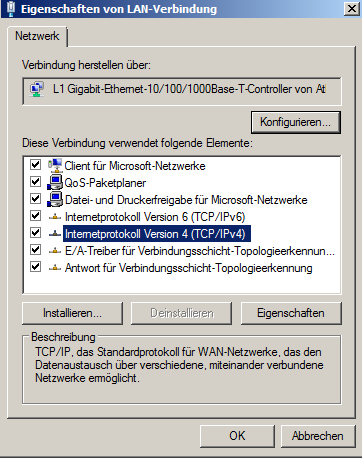
\includegraphics[height=7cm]{Bilder/004}\\ \end{center}
	
In dem folgenden Dialog können wir dann die IP-Adresse des Rechners festlegen.\\ 

	\begin{center}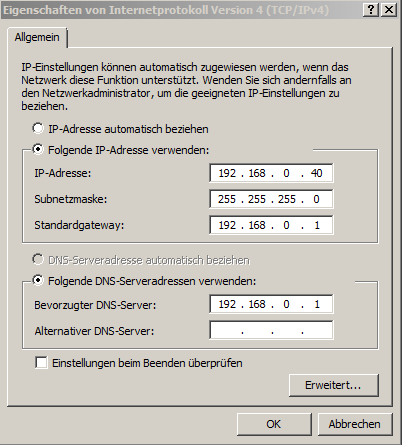
\includegraphics[height=7cm]{Bilder/005}\\ \end{center}
	
Dazu stellen wir den Radiobutton auf \emph{Folgende IP-Adresse verwenden} und geben dann eine in dem lokalen Netzwerk von keinem anderen Rechner benutzte IP-Adresse an, mit der passenden Subnetzmaske. als Standardgateway dient üblicherweise der Netzwerkrouter. Den DNS-Server müssen wir nun auch von Hand eingeben, dieser läuft üblicherweise auch auf dem Netzwerkrouter.\\
Damit wären die Vorarbeiten abgeschlosen, als nächstes wird die Active Directory-Domänendienste Rolle installiert.

\newpage
\section{Active Directory-Domänendienste installieren}
Zum installieren der Active Directory-Domänendienste öffnen wir wie zum installieren jeder anderen Rolle den \emph{Server Manager}. Standardmäßig findet sich dieser in der Taskleiste. In der \emph{Rollenübersicht} wählen wir \emph{Rollen hinzufügen} um die Rolle Active Directory-Domänendienste zu installieren.\\

	\begin{center}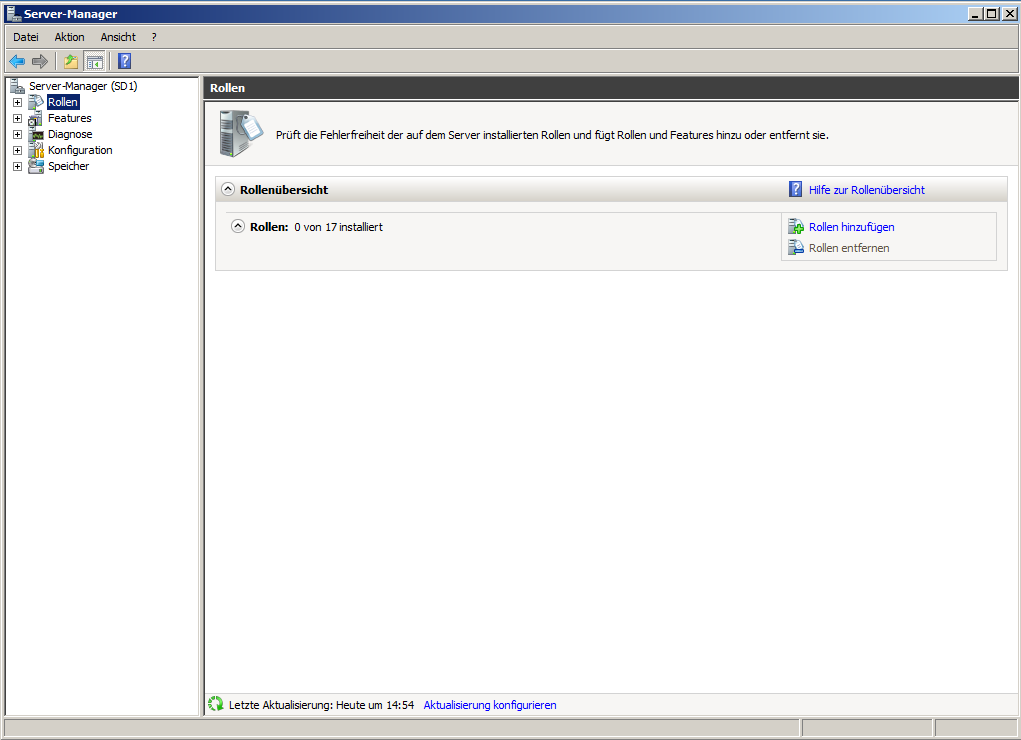
\includegraphics[width=14cm]{Bilder/006}\\ \end{center}
	
Den Bildschirm mit den Vorbemerkungen mit einem Klick auf \emph{Weiter} zur Kenntnis nehmen. Im \emph{Serverrollen auswählen} Dialog wählen wir \emph{Active Directory-Domänendienste} aus und klicken auf \emph{Weiter}.\\

	\begin{center}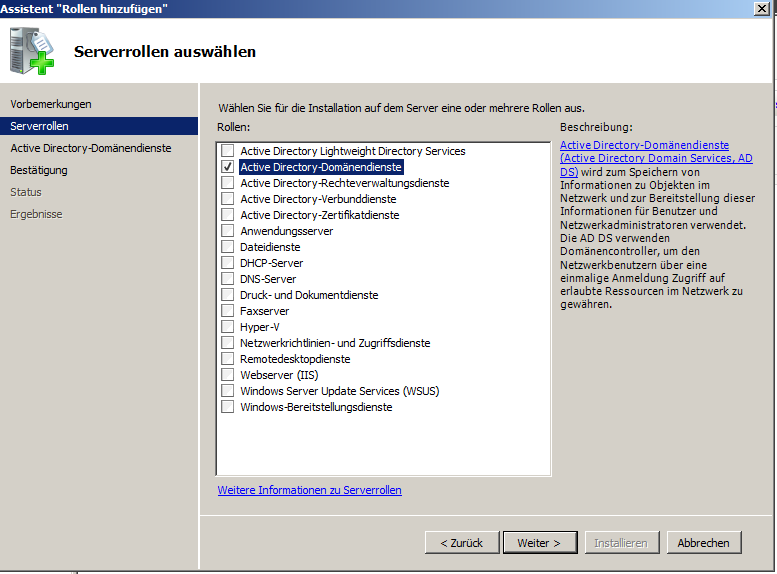
\includegraphics[height=9cm]{Bilder/008}\\ \end{center}
	
Die anderen Rollen die wir später noch installieren wollen können wir jetzt noch nicht installieren da Windows erst die Active Directory-Domänendienste Rolle komplett konfigurieren will bevor man weitere Rollen installieren darf.\\
 
 	\begin{center}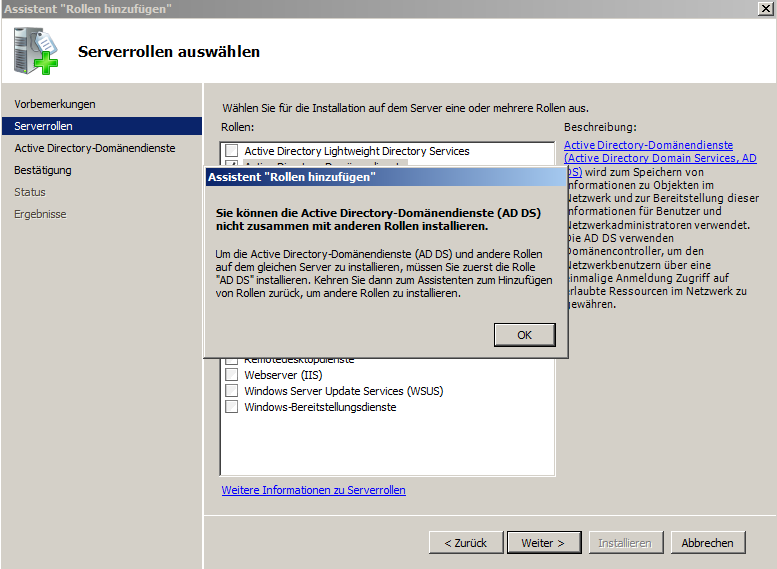
\includegraphics[height=9cm]{Bilder/009}\\ \end{center}
 	
Wenn es nicht bereits installiert ist will der Server Manager das benötigte .NET Framework 3.5.1 noch mitinstallieren. Den \emph{Einführung in die Active Directory-Domänendienste} Dialog durchlesen und mit einem Klick auf \emph{Weiter} zur Kenntnis nehmen. Daraufhin erhalten wir eine Übersicht der zu installierenden Rollen und Features, die wir mit einem Klick auf \emph{Installieren} bestätigen.\\

 	\begin{center}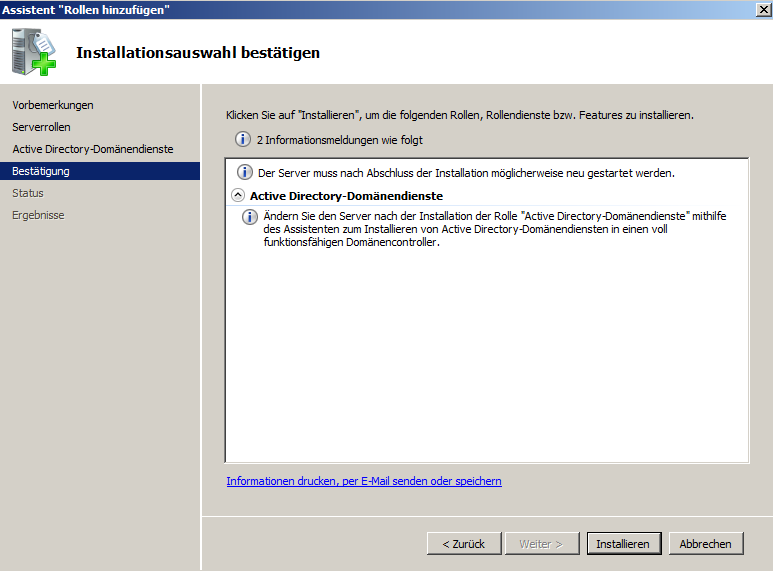
\includegraphics[height=9cm]{Bilder/011}\\ \end{center}
 
Daraufhin installiert Windows die Rollen und Features, dies kann einige Minuten in Anspruch nehmen. Zum Abschluss erscheint der \emph{Installationsergebnisse} Dialog, der für alles eine erfolgreiche Installation melden sollte. Danach muss der Active Directory-Domänendienst eingerichtet werden.
 
 \newpage
 \section{Active Directory-Domänendienste einrichten}
Um die Active Directory-Domänendienste einzurichten rufen wir dcpromo.exe auf.\\

	\begin{center}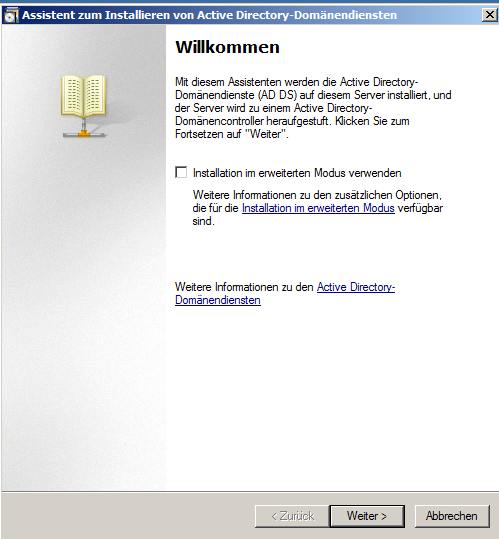
\includegraphics[height=7cm]{Bilder/014(dcpromo_exe01)}\\ \end{center}
	
Der Hinweis zur Betriebssystemkompatibilität kann von uns hier ignoriert werden, sollte aber trotzdem durchgelesen und dann mit \emph{Weiter} abgenickt werden. In dem darauffolgenden Dialog wählen wir \emph{Neue Domäne in neuer Gesamtstrutktur erstellen} da wir über keine bestehende Domäne verfügen die wir verwenden wollen.\\

	\begin{center}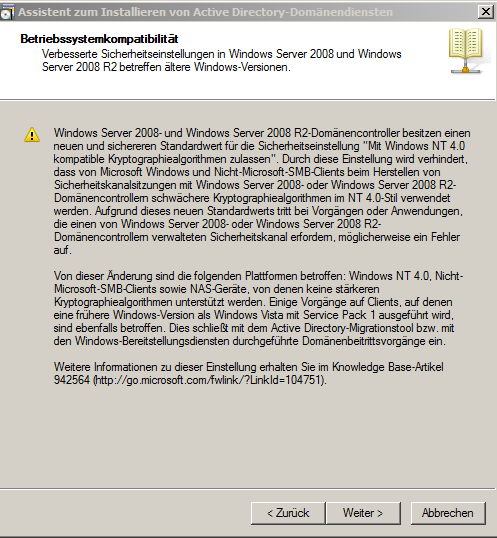
\includegraphics[height=7cm]{Bilder/015(dcpromo_exe02)}\\ \end{center}
	
Als nächstes muss der Fully Qualified Domain Name (\emph{FQDN}) der neuen Domäne angegeben werden. Da wir keine internetfähige Domäne verwalten wollen geben wir einen Namen an der auf \emph{.local} endet.\\

	\begin{center}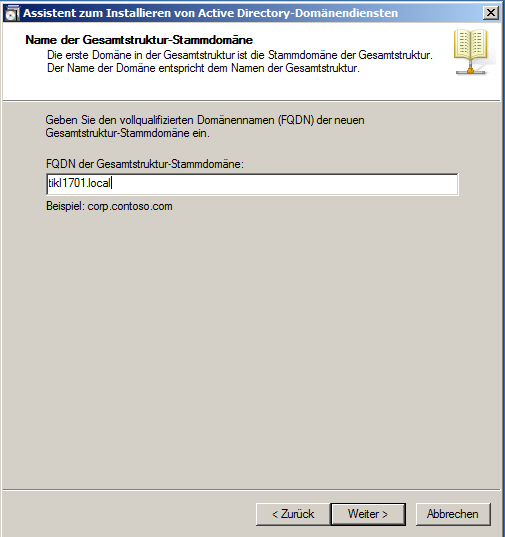
\includegraphics[height=7cm]{Bilder/017(dcpromo_exe04)}\\ \end{center}
		
Nach dem klicken auf \emph{Weiter} wird geprüft ob der angegebene Name schon verwendet wird. Als nächstes sollen wir die Funktionsebene der Gesamtstruktur festlegen. Da wir die Domäne komplett neu aufsetzen wählen wir das neueste verfügbare, also \emph{Windows Server 2008 R2}.\\

	\begin{center}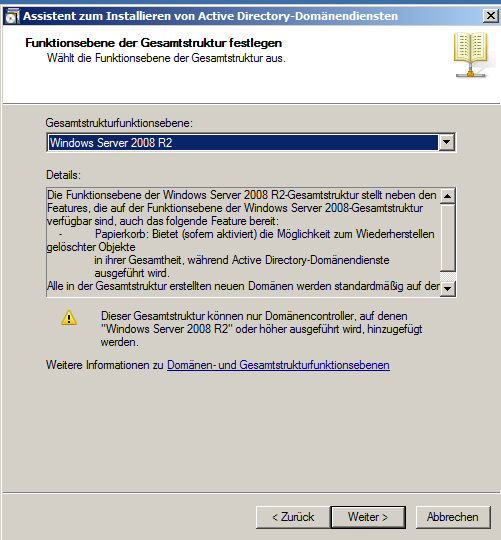
\includegraphics[height=7cm]{Bilder/019(dcpromo_exe06)}\\ \end{center}
	
Nach einem Klick auf \emph{Weiter} wird erst die vorhanden DNS-Konfiguration geprüft, danach erscheint der Dialog \emph{Weitere Domänencontrolleroptionen}.\\

	\begin{center}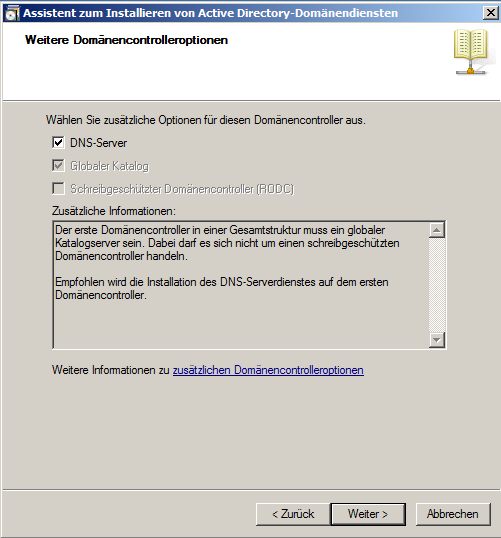
\includegraphics[height=7cm]{Bilder/021(dcpromo_exe08)}\\ \end{center}

Da wir später auch noch einen \emph{DNS-Server} aufsetzen wollen wählen wir diese Option aus. Da wir den ersten Domain Controller der Domäne einrichten muss die Option \emph{Globaler Katalog} zwingend aktiviert sein und darf auch nicht deaktiviert werden. Aus demselben Grund kann die Option \emph{Schreibgeschützer Domänencontroller (RODC)} nicht aktiviert werden.\\
Nach einem Klick auf \emph{Weiter} erscheint eine Fehlermeldung da wir den DNS-Server noch nicht eingerichtet haben und kein übergeordneter DNS-Server verfügbar ist.\\

	\begin{center}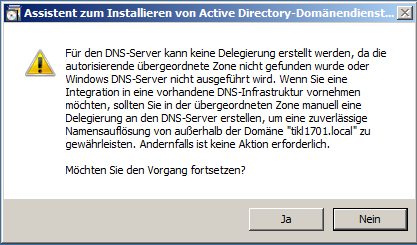
\includegraphics[height=7cm]{Bilder/022(dcpromo_exe09)}\\ \end{center}
	
Den Dialog mit \emph{Ja} bestätigen.\\
Danach wird nach den Speicherorten für Datanbank, Protokolldateien und SYSVOL gefragt. Da wir nichts an den Standardorten ändern wollen bestätigen wir das Ganze einfach mit \emph{Weiter}.\\
Danach müssen wir dem Administratorkonto für die Domäne ein Kennwort vergeben, nach den üblichen Richtlinien (mindestens 8 Stellen, mindestens 1 Buchstabe, mindestens 1 Zahl). Hier sollte ein möglichst sicheres Kennwort gewählt werden. Dies eintragen und nochmal zur Bestätigung eintragen, danach \emph{Weiter} wählen.\\
Nun wird eine Zusammenfassung unserer Einstellungen angezeigt bevor diese ausgeführt werden. Hier könnten wir diese Einstellungen durch klicken auf \emph{Einstellungen exportieren} falls wir dieselben Einstellungen auf mehreren Rechnern ausführen wollen würden. Aber dies ist bei dem primären Domaincontroller nicht allzu sinnvoll und auch nicht Ziel diese Dokumentation. Nach der Bestätigung mit \emph{Weiter} richtet Windows den Domänencontroller ein. Dies kann einige Minuten in Anspruch nehmen.\\
Sobald alles eingerichtet ist beenden wir den Assistenten mit einem Klick auf \emph{Fertig stellen}, danach muss der Server neu gestartet werden. Dies schließt auch die Installation des Active Directory-Domänendienste ab.

\newpage
\section{DNS-Server installieren und einrichten}
Zuerst einmal muss hierfür die DNS-Server Rolle im \emph{Server Manager} installiert werden. Dies geht analog zur Installation der Active Directory-Domänendienste Rolle aus Kapitel 2. Danach öffnen wir die DNS Einstellungen im Server Manager und klappen den Baum so lange auf bis wir den Punkt \emph{Reverse-Lookupzonen} sehen.\\

	\begin{center}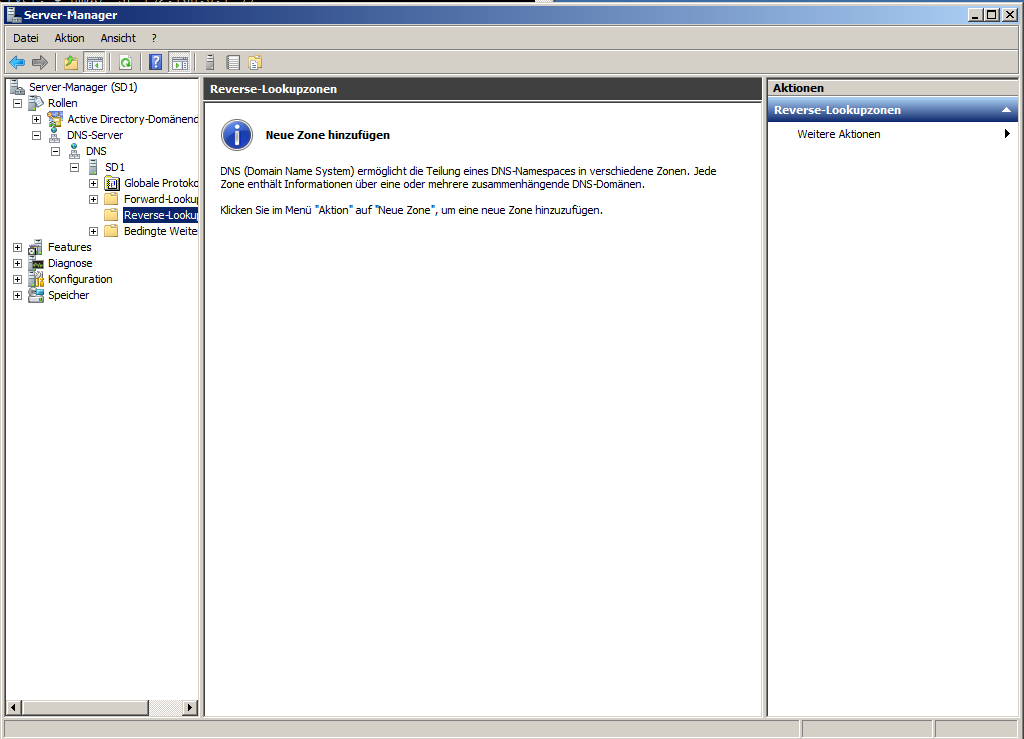
\includegraphics[height=9cm]{Bilder/029(DNS01)}\\ \end{center}

Um eine neue Reverse-Lookupzone zu erstellen wählen wir diesen Punkt mit der rechten Maustaste an und wählen \emph{Neue Zone} aus.\\
Den Willkommensbildschirm nehmen wir mit der Auswahl von \emph{Weiter} zur Kenntnis. Als nächstens wählen wir die vorausgewählte Option \emph{Primäre Zone} da dies die erste (und vorerst die einzige) Zone ist die wir erstellen. Mit \emph{Weiter} bestätigen. Auch im nächsten Bildschirm wählen wir für die Zonenreplikation die vorausgewählte Option \emph{Auf allen Servern, die auf Domänencontrollern in dieser Domäne ausgeführt werden: \textit{Domänenname}} (in unserem Beispiel tikl1701.local). \emph{Weiter} führt auch hier... weiter. In unserem Beispiel arbeiten wir mit IPv4 Adressen, deswegen wählen wir im nächsten Bildschirm wieder die Voreinstellung \emph{IPv4 Reverse-Lookupzone}.\\
Die Auswahl von \emph{Weiter} führt wie fast immer zum nächsten Dialog in welchen nun der \emph{Name der Reverse-Lookupzone} angegeben werden soll.\\

	\begin{center}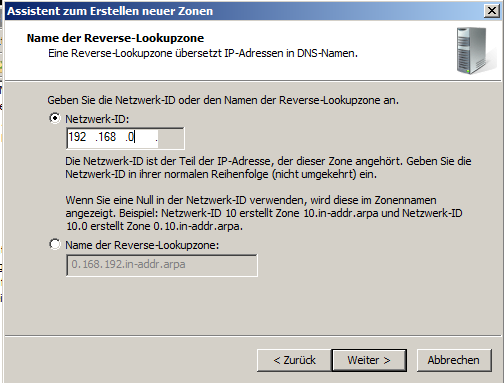
\includegraphics[height=7cm]{Bilder/034(DNS06)}\\ \end{center}
	
Hier muss nun die Netzwerk-ID angeben werden, also in unserem Beispiel die 192.168.0. Die Auswahl von \emph{Weiter} führt zu Dialog \emph{Dynamisches Update}. Hier wählen wir \emph{Nur sichere dynamische Updates zulassen} da dies die empfohlene Option für Active Directory ist.\\
Die Auswahl von \emph{Weiter} führt uns auch schon zum \emph{Fertigstellen des Assistenten} Dialogs, der nochmal die vorzunehmenden Einstellungen zusammenfasst. Dieser wird dann mit \emph{Fertig stellen} beendet.\\

	\begin{center}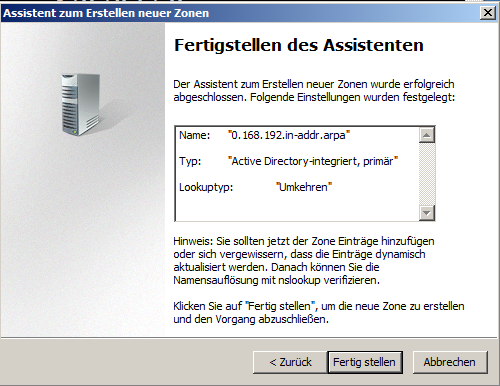
\includegraphics[height=7cm]{Bilder/036(DNS08)}\\ \end{center}

Als nächstes wählen wir im \emph{Server Manager} den eigenen Rechnernamen mit der rechten Maustaste aus und wählen dort \emph{Eigenschaften}. Hier kontrollieren wir ob im Reiter \emph{Weiterleitungen} der DNS-Server des Netzes für externe Anfragen eingetragen ist. Normalerweise wurde dies schon vom Assistenten erledigt, falls nicht muss sie durch Klick auf \emph{Bearbeiten} eingetragen werden.\\

	\begin{center}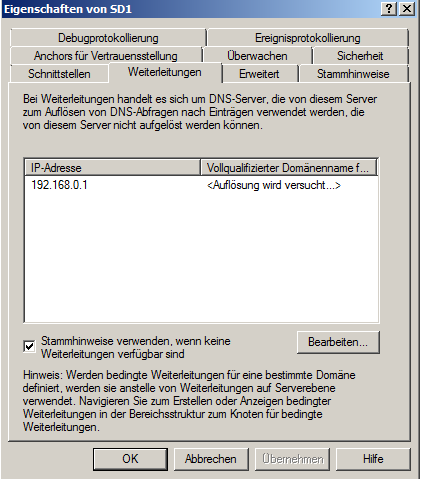
\includegraphics[height=7cm]{Bilder/038(DNS10)}\\ \end{center}

Somit ist die Einrichtung des DNS-Servers abgeschlossen, als nächstes wird der DHCP-Server eingerichtet.

\newpage
\section{DHCP-Server installieren und einrichten}
Zuerst einmal muss die DHCP-Server Rolle mit dem \emph{Server Manager} installiert werden, analog zur Active Directory-Domänendienste Rolle in Kapitel 2.\\

	\begin{center}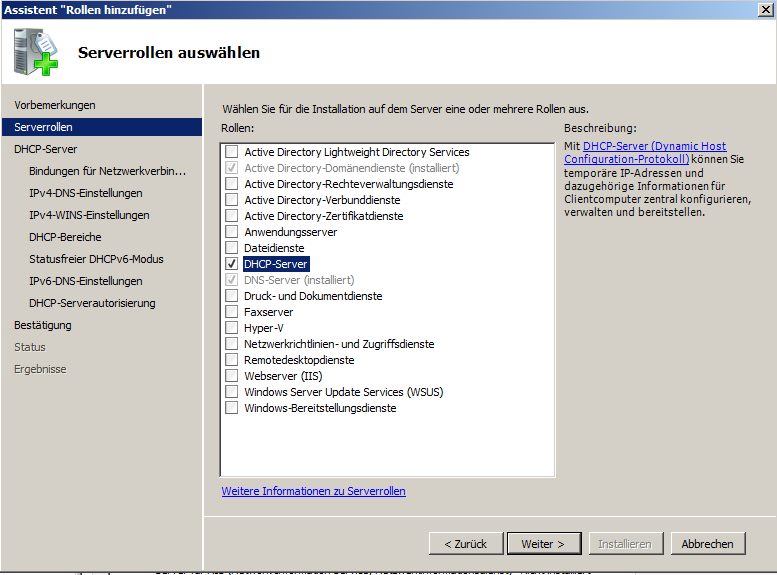
\includegraphics[height=9cm]{Bilder/039(DHCP01)}\\ \end{center}

Die allgemeinen Hinweise zu DHCP-Servern, ebenso wie die vorherige Auswahl, bestätigen wir mit einem Klick auf \emph{Weiter}. Als nächstes müssen wir den Namen unserer Domäne angeben und unseren DNS-Server. Da wir den DNS-Server auf demselben Rechner laufen lassen geben wir hier die IP von localhost (127.0.0.1) an. Des weiteren empfiehlt es sich den DNS-Server des lokalen Netzes als alternativen Server anzugeben.Das Ganze mit \emph{Weiter} bestätigen.\\

	\begin{center}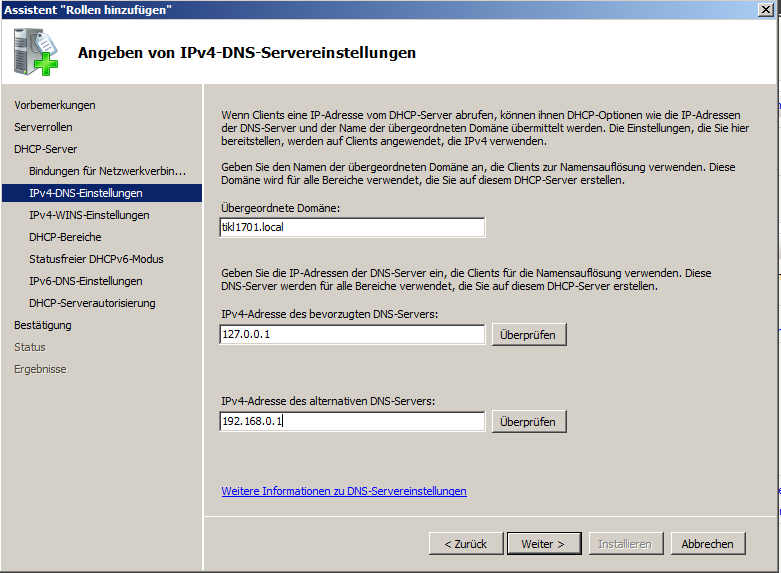
\includegraphics[height=9cm]{Bilder/041(DHCP03)}\\ \end{center}
	
Da wir kein WINS verwenden wollen wählen wir im nächsten Dialog die Option \emph{WINS ist für Anwendungen in diesem Netzwerk nicht erforderlich} und bestätigen dies mit \emph{Weiter}. Als nächstes sollen wir auswählen welche IPs der DHCP Server verteilen soll. Dazu klicken wir auf \emph{Hinzufügen}. Daraufhin erscheint das Fenster zum Hinzufügen eines Adressbereiches.\\

	\begin{center}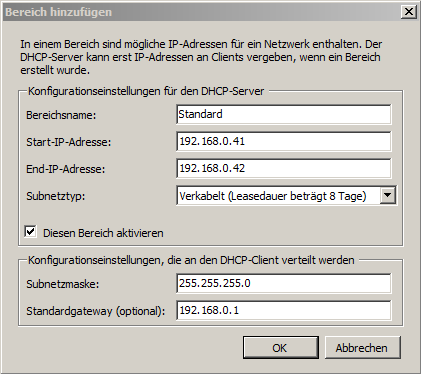
\includegraphics[height=7cm]{Bilder/043(DHCP05)}\\ \end{center}
	
Hier tragen wir einen möglichst gut \emph{identifizierbaren Namen} für den Bereich, die \emph{Start- und End-IP-Adresse} des Bereichs und die \emph{Leasedauer} ein. Die Leasedauer kann vorerst auf 8 Tage gesetzt werden solange dies nicht irgendwelche Probleme aufwirft. Unten geben wir noch die \emph{Subnetzmaske} und das lokale \emph{Gateway} an damit die Clients diese Einstellung richtig verteilt bekommen.\\	
Bei dem Ganzen ist darauf zu achten das aus dem IP-Bereich keine Adressen bereits verwendet (oder von einem anderen DHCP verteilt) werden und der Haken bei \emph{Diesen Bereich aktivieren} gesetzt ist. Nach dem Bestätigen mit \emph{Ok} könnten wir noch andere Adressbereiche hinzufügen, aber in diesem Beispiel verwenden wir nur einen. Deswegen klicken wir auf \emph{Weiter}.\\
Die IPv6-Optionen in den nächsten 2 Bildschirmen lassen wir auf den Standardwerten stehen da diese bereits richtig eingestellt sind und wir uns hier auf IPv4 kontentrieren. Zuletzt müssen wir noch die Serverautorisierung angeben. Da wir auch den Domänencontroller auf demselben Rechner verwalten wählen wir die Option \emph{Aktuelle Anmeldeinformationen verwenden}.\\
Im letzten Dialog erhalten wir wieder eine Übersicht über die vorzunehmende Installation und Konfiguration, mit dem Button \emph{Installieren} wird der Vorgang gestartet.\\ 

	\begin{center}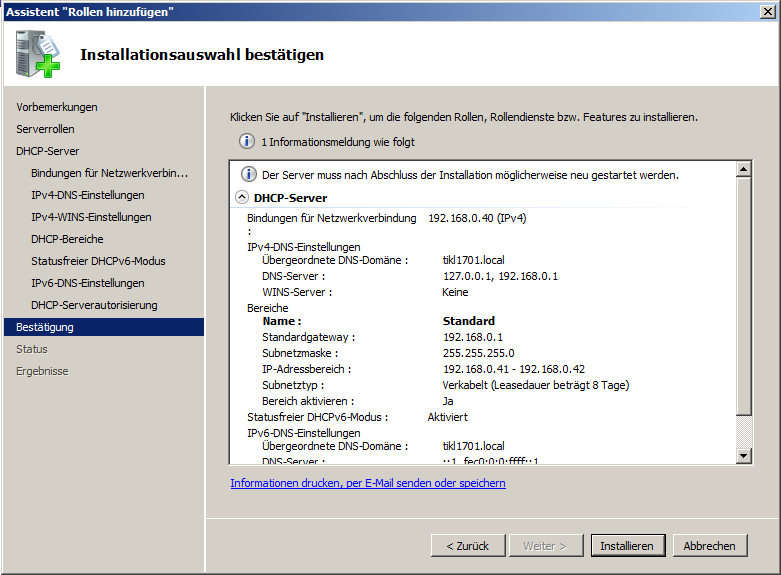
\includegraphics[height=9cm]{Bilder/048(DHCP10)}\\ \end{center}
	
Nach ein paar Minuten sollte die Installation erfolgreich abgeschlossen sein, als nächstes legen wir Benutzer für unsere Domäne an.

\newpage
\section{Domänenbenutzer anlegen}
Um Domänenbenutzer anzulegen rufen wir zuerst Active Directory-Benutzer und -Computer Verwaltungskonsole unter \emph{Start \ding{221} Verwaltung \ding{221} Active Directory-Benutzer und -Computer} auf. Hier klappen wir den Baum unter unserer Domäne auf und wählen im Kontextmenü von \emph{Users} den Punkt \emph{Neu \ding{221} Benutzer}. In das darauf erscheinende Fenster tragen wir die diversen Namen des Benutzers ein (Vor- und Nachname und Anmeldename).\\

	\begin{center}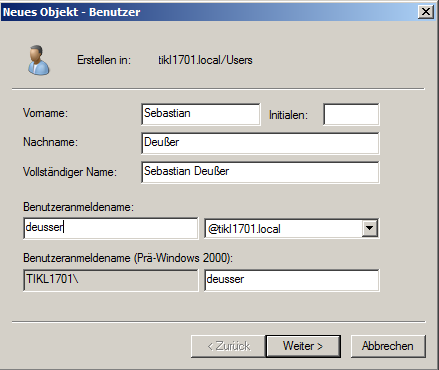
\includegraphics[height=7cm]{Bilder/050}\\ \end{center}
	
Auf der nächsten Seite muss dem Benutzer ein den Kennwortrichtlinien entsprechendes Passwort zugewiesen werden. Die Option \emph{Benutzer muss Kennwort bei der nächsten Anmeldung ändern} sollte aktiviert werden, damit der Anwender beim ersten Anmelden aufgefordert wird ein persönlicheres Passwort zu vergeben.\\

	\begin{center}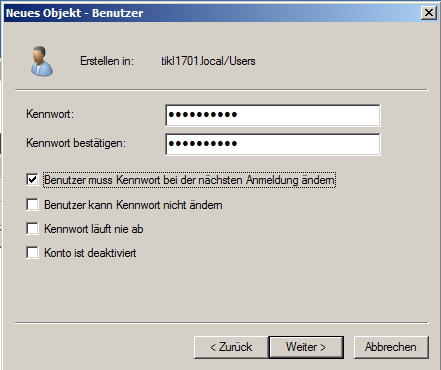
\includegraphics[height=7cm]{Bilder/051}\\ \end{center}
	
Auf der letzten Seite erhalten wir noch eine Übersicht über die angegebene Daten, mit einem Klick auf \emph{Fertig stellen} wird der Benutzer erstellt.
Will man einem Benutzer zusätzlich Administratorenrechte geben, so sucht man den Benutzer im rechten Teil der Active Directory-Benutzer und -Computer Verwaltungskonsole (nach Auswahl von Users) und wählt im Kontextmenü des Benutzernamens den Punkt \emph{Eigenschaften}. Reiter \emph{Mitglied von} kann man den Benutzer über den Button \emph{Hinzufügen...} Mitglied neuer Gruppen werden lassen.\\

	\begin{center}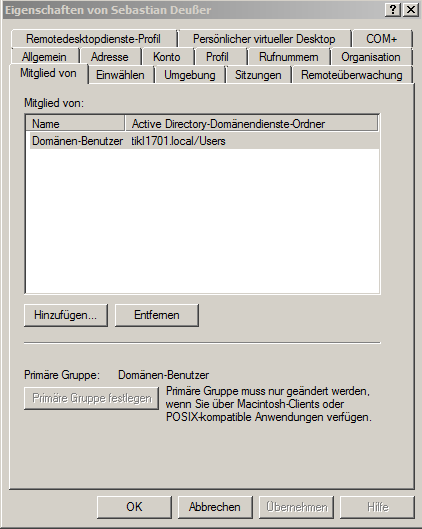
\includegraphics[height=7cm]{Bilder/052}\\ \end{center}
	
In den Dialog danach gibt man dann den Namen der gewünschten Gruppe (oder den eindeutigen Anfang des Namens) an und klickt auf \emph{Namen überprüfen}.\\
	
	\begin{center}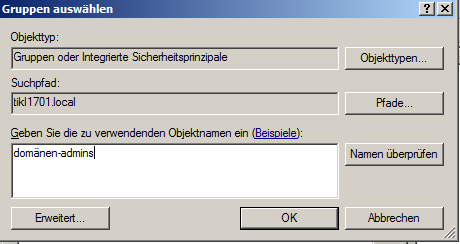
\includegraphics[height=3.5cm]{Bilder/053}\\ \end{center}
	
Die für uns hier interessanten Gruppen sind \emph{Adminstratoren} (die Gruppe der Benutzer mir Administratorrechten auf diesem Rechner) und \emph{Domänen-Admins} (Benutzer die Administratorenrechte für die Domäne und alle Mitglieds-Rechner besitzen).\\
Zuletzt wollen wir noch einen Rechner unserer Domäne hinzufügen.

\newpage
\section{Client-Rechner der Domäne hinzufügen}
Als letztes wollen wir noch einen Windows 7 Client-Rechner unserer Domäne hinzufügen.\\
Hierzu müssen wir zuerst den DNS-Server unserer Domäne als bevorzugten DNS-Server eintragen. Dazu rufen wir \emph{Systemsteuerung \ding{221} Netzwerk und Internet \ding{221} Netzwerk- und Freigabecenter} auf und rufen in den Adaptereigenschaften unserer Netzwerkkarte die \emph{Eigenschaften} von \emph{Internetprotokoll Version 4 (TCP/IPv4)} auf. Dort tragen wir in unserem Fall folgendes ein:\\

	\begin{center}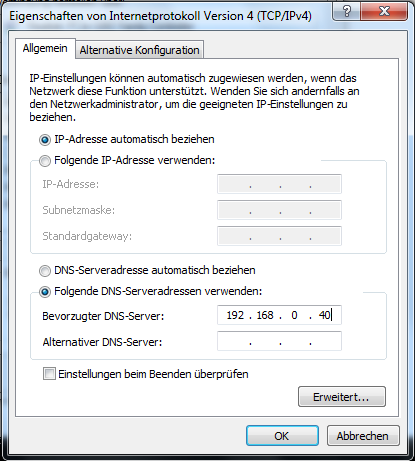
\includegraphics[height=7cm]{Bilder/Client/Client01}\\ \end{center}
	
Als nächstes rufen wir wie in Kapitel 1 über den Punkt \emph{Eigenschaften} im Kontextmenü von Computer (z.B. in der Sidebar des Startmenüs) die Basisinformationen des Systems auf. Wieder wählen wir \emph{Einstellungen ändern}. In dem Fenster das sich daraufhin öffnet klicken wir den Button \emph{Ändern} an. Es öffnet sich der Dialog den wir schon aus Kapitel 1 kennen.\\

	\begin{center}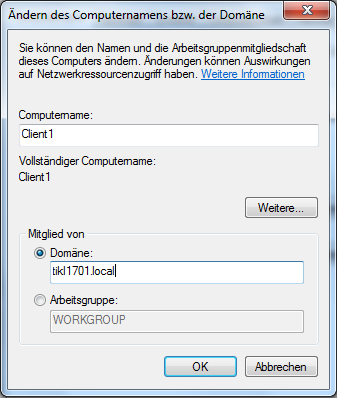
\includegraphics[height=7cm]{Bilder/Client/Client03}\\ \end{center}
	
Hier tragen wir nun unsere neue Domäne ein. Danach fragt Windows nach dem Benutzernamen und Passwort eines Benutzerkontos das der Domäne beitreten darf.\\

	\begin{center}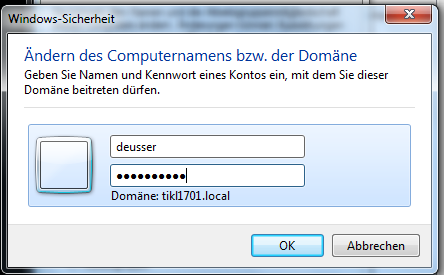
\includegraphics[height=4cm]{Bilder/Client/Client04}\\ \end{center}

Hier tragen wir z.B. einen unserer in Kapitel 6 neu erstellten Benutzer ein. Nach richtiger Eingabe der Daten erscheint die Willkommensmeldung zu Domäne.\\

	\begin{center}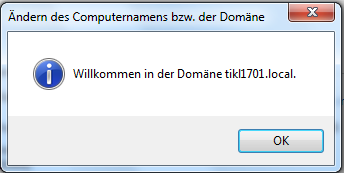
\includegraphics[width=6.5cm]{Bilder/Client/Client05}\\ \end{center}
	
Gefolgt wird diese von Aufforderungen zum Begrüßungsneustart.\\

	\begin{center}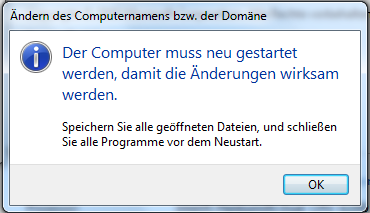
\includegraphics[width=6.5cm]{Bilder/Client/Client06}\\ \end{center}
	
	\begin{center}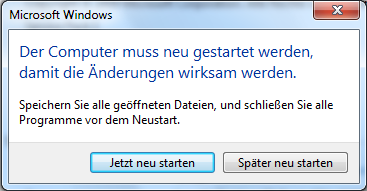
\includegraphics[width=6.5cm]{Bilder/Client/Client07}\\ \end{center}

Nach dem durchführen des Neustarts können wir uns dann mit dem Benutzerkonto eines Domänenbenutzers anmelden. Dazu müssen wir noch das richtige Benutzerkonto über auswählen von \emph{Benutzer wechseln \ding{221} Anderes Benutzerkonto} auswählen. Die Domäne ist in der Eingabemaske dann schon voreingestellt.\\
Die Eingabe korrekter Zugangsdaten vorrausgesetzt können wir nun mit dem Client in unserer neuen Domäne arbeiten.
\end{document}
